\subsection{Product perspective}

\subsubsection{Class Diagram} %%done !!!!!!!!!!!!!!!!!!
The following class diagram is a high-level class diagram which should be intended as a model of the application structure. During the implementation part more classes and attributes can be created and used.

%Sideway figure
%\begin{sidewaysfigure}
%\centering
%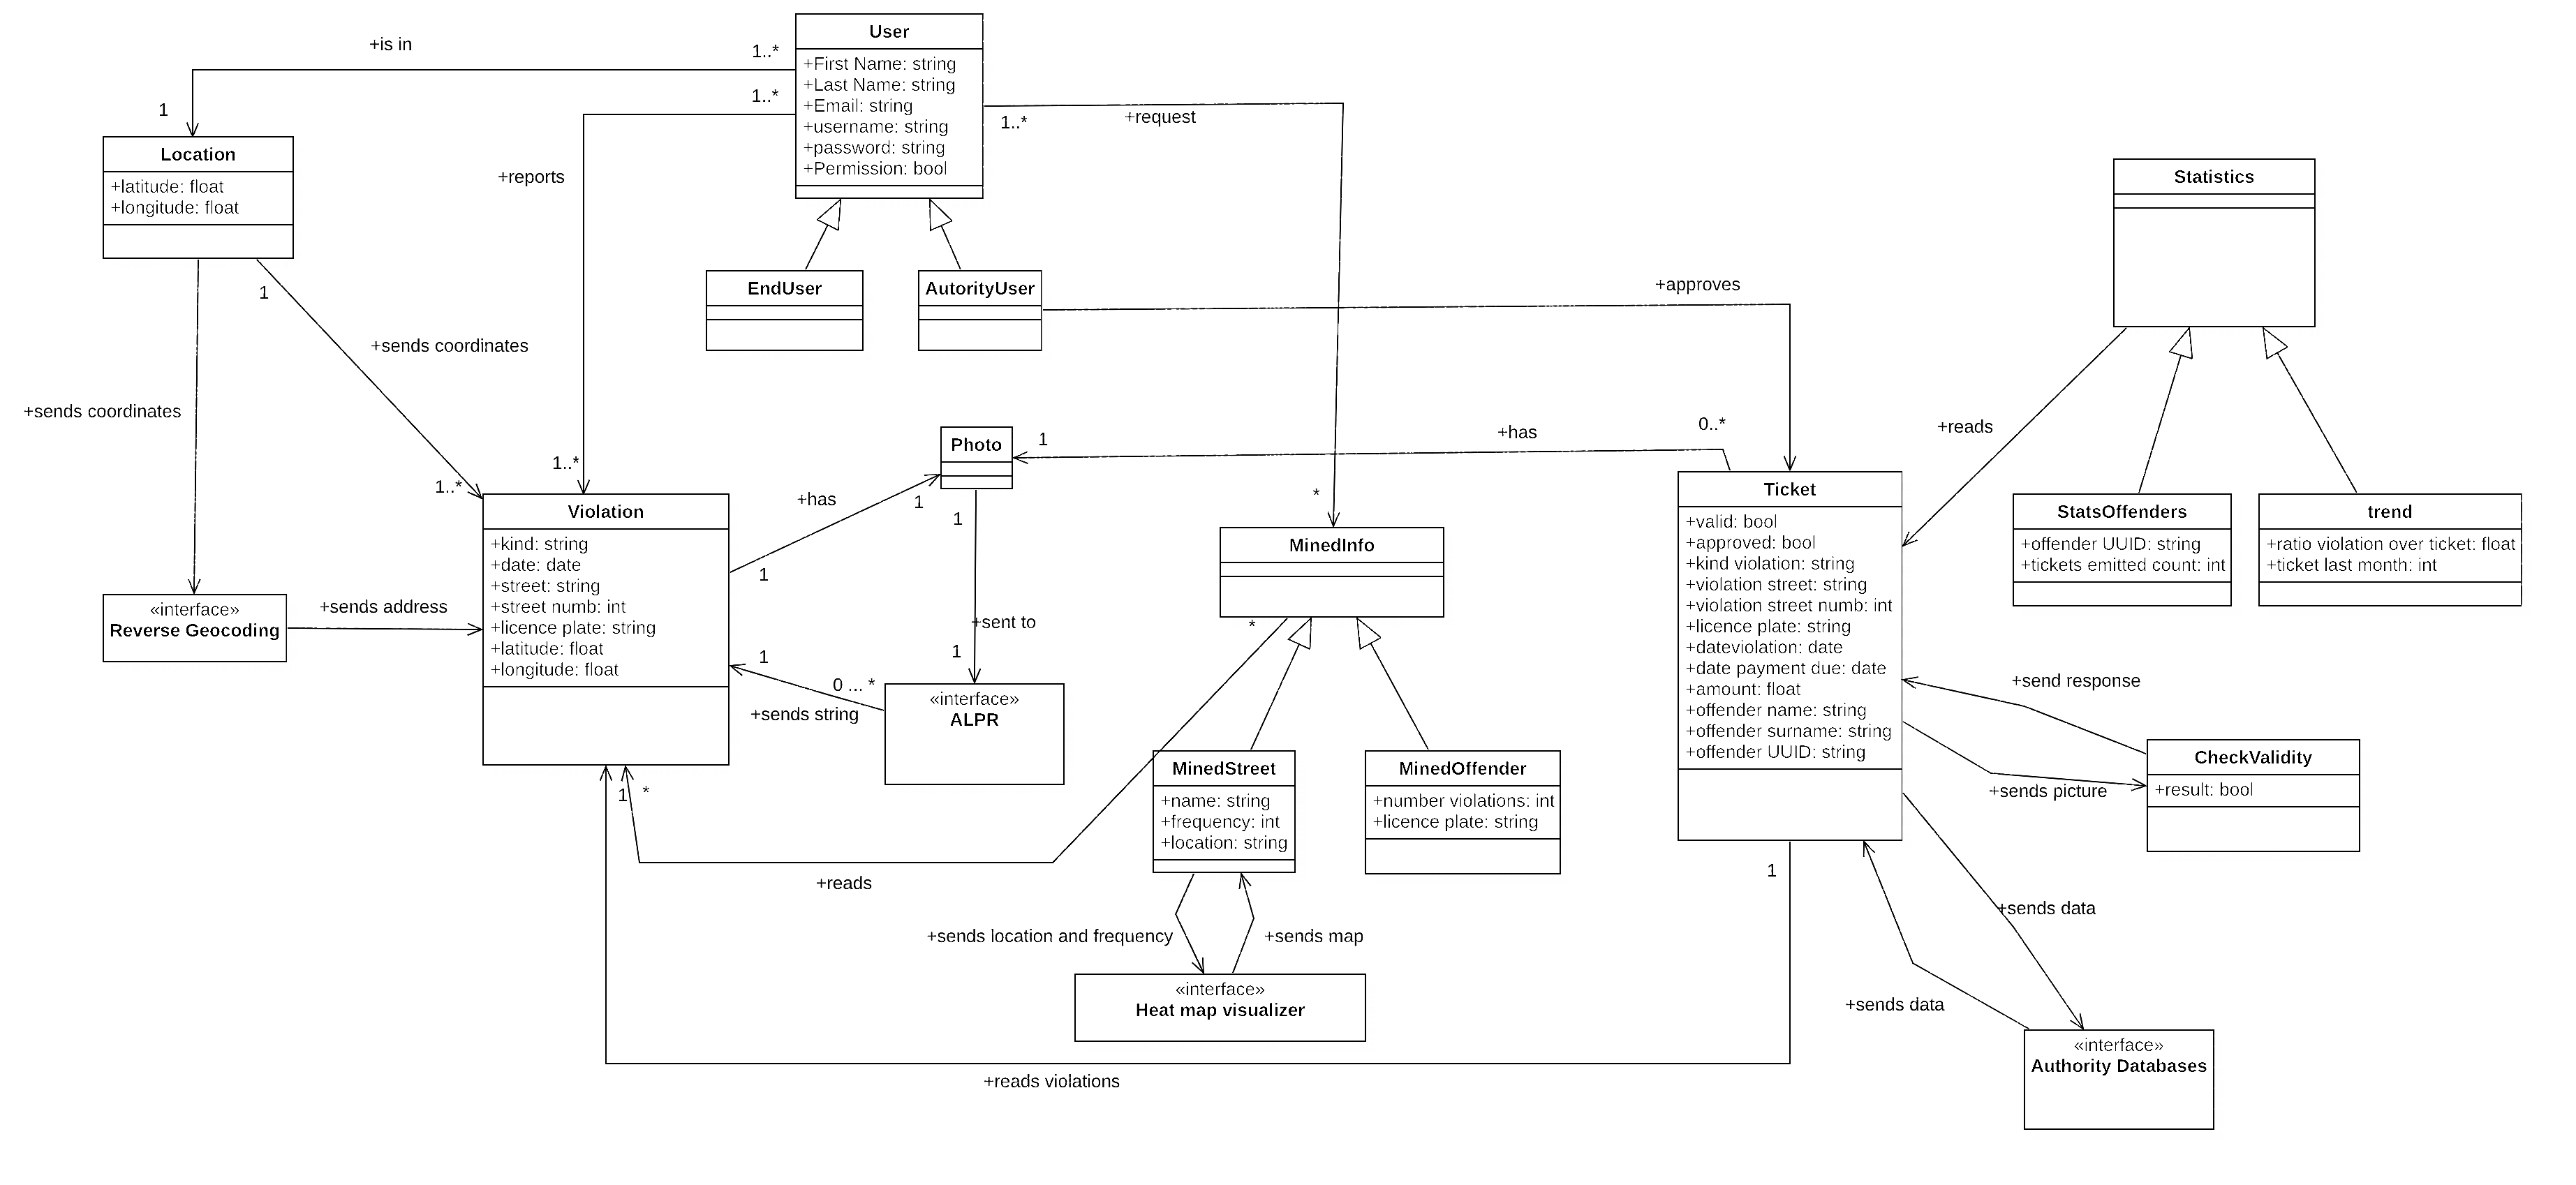
\includegraphics[width=\textwidth]{Images/Class.png}
%\caption{\label{fig:classdiagram}High-level Class Diagram}
%\end{sidewaysfigure}

\begin{sidewaysfigure}
\centering
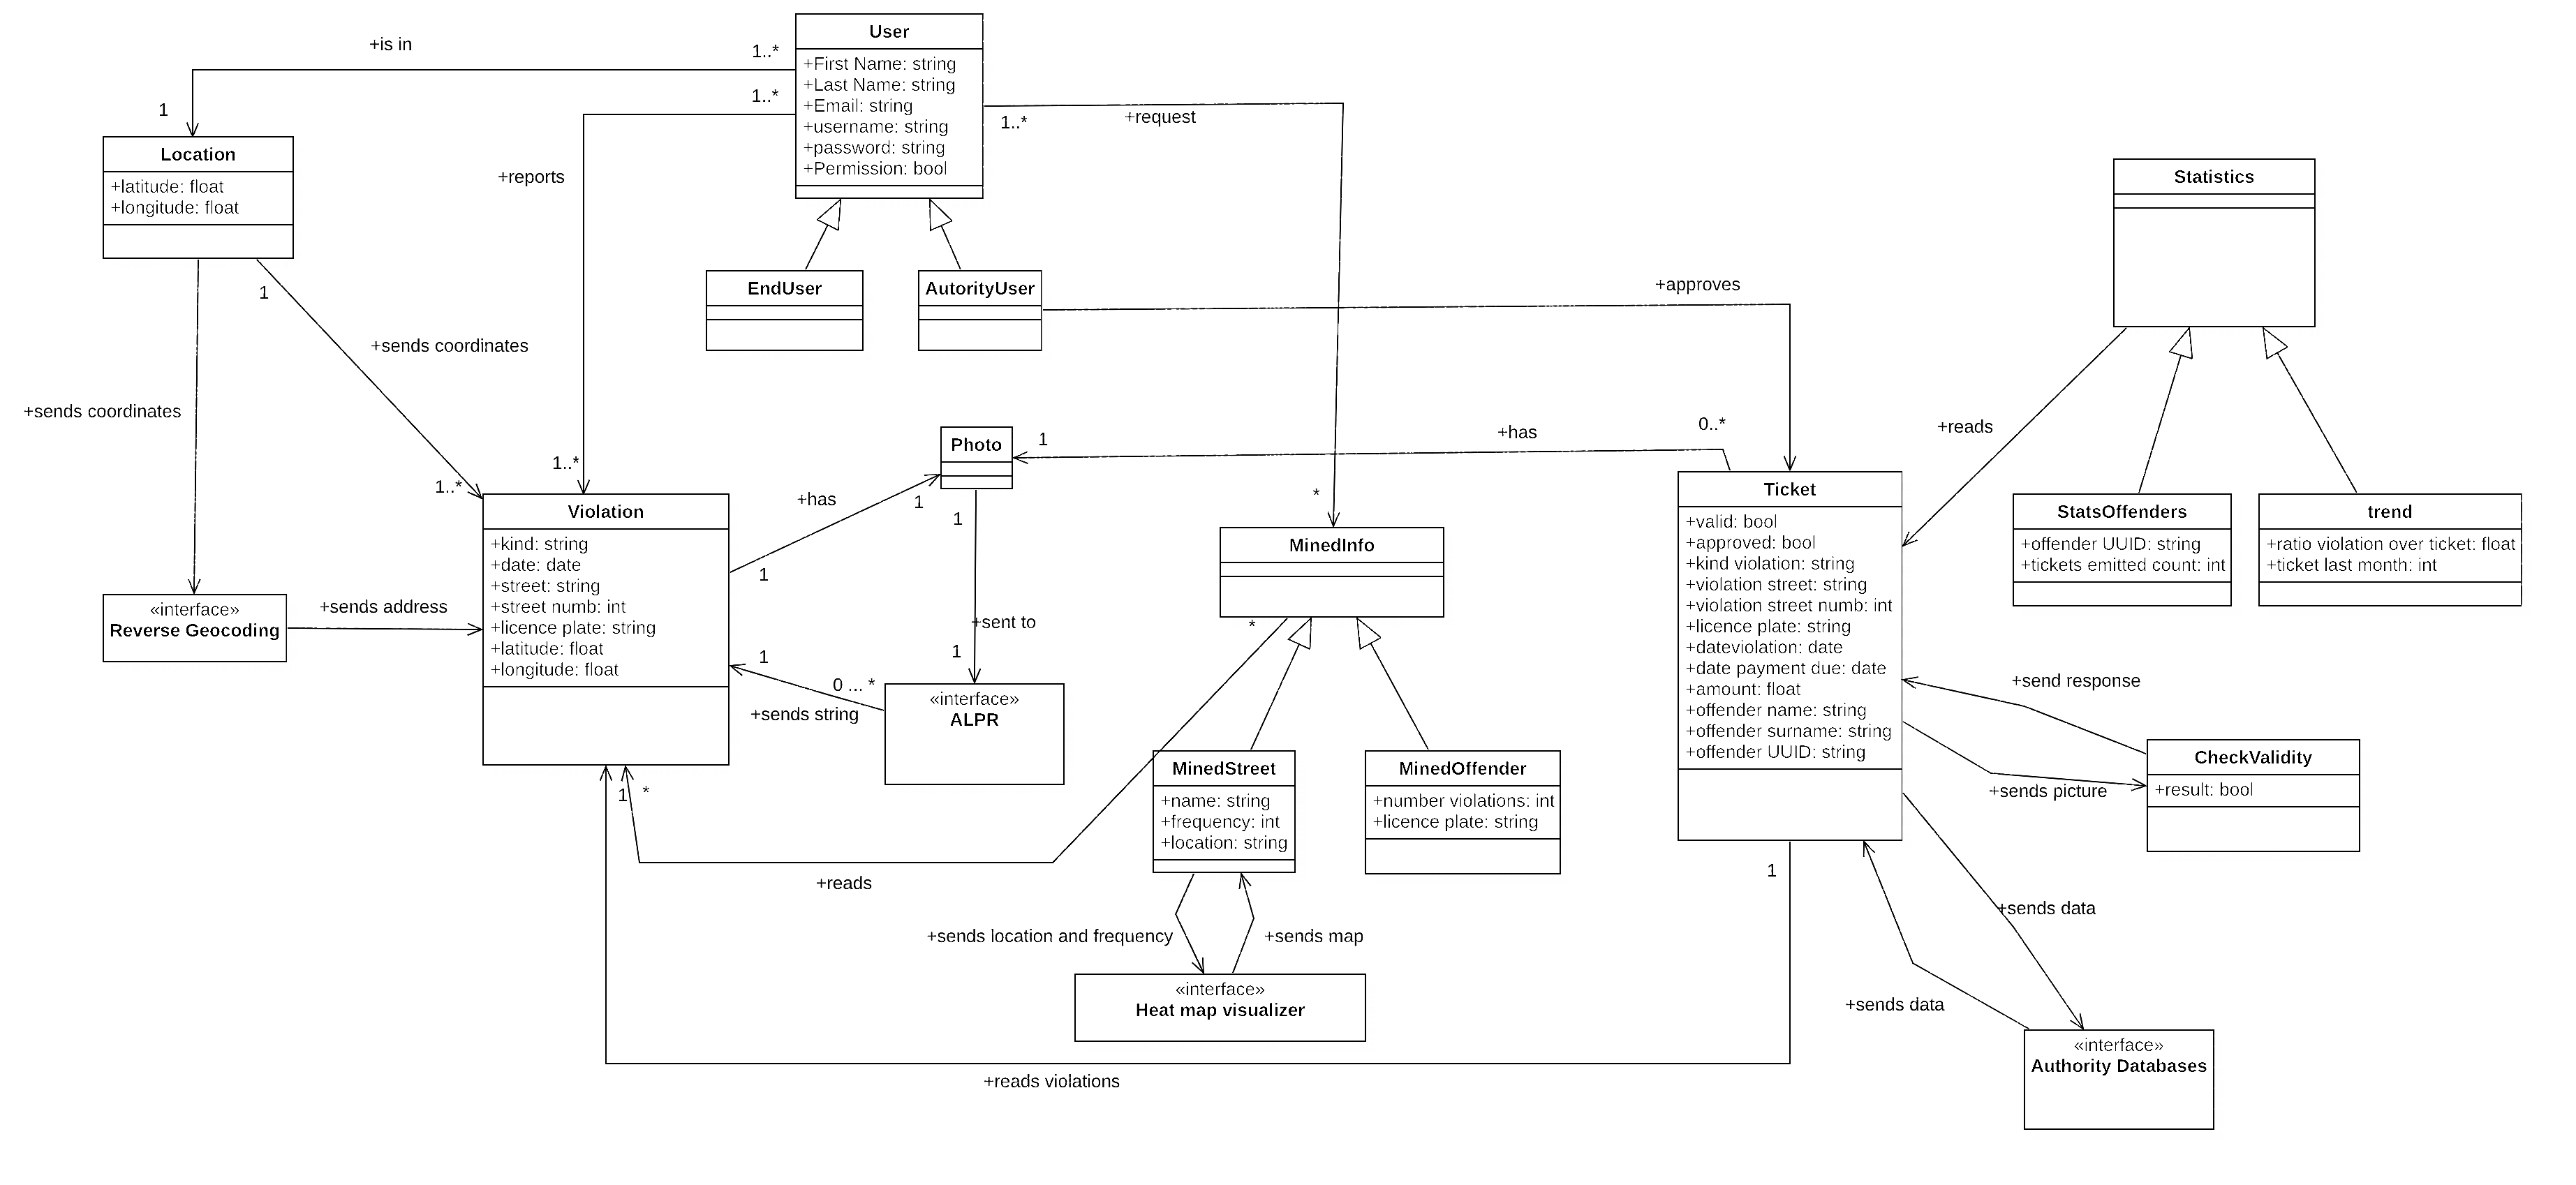
\includegraphics[width=\textwidth]{Images/Class.png}
\caption{\label{fig:classdiagram}High-level Class Diagram}
\end{sidewaysfigure}

\paragraph{User}
This class is the father of the two possible kind of users: \textbf{EndUser} and \textbf{Authority}, which are needed because our application is intended to be multi-user and with at least two privileges for data that can be viewed and possible functions accessible.

\paragraph{Location}
Every user is in a \textbf{Location} class used to represent the location as latitude and longitude coming from the OS of the smartphone.

\paragraph{Reverse Geocoding}
This interface is used to communicate with the external Geocoding service to get a readable address from the coordinates as explained in section \ref{Dependencies}.

\paragraph{Violation}
This class is used to store all the data related to the reported violation. The \textit{kind} attribute is selected by the user from a list of possible kind of violations in the form section as explained in \ucas{4b}.  In the \textbf{Violation} class we store also the raw latitude and longitude in case there will be need of those data later, as an example if it's imposssible get a precise address using reverse geocoding.

\paragraph{Photo}
This class is needed to represent the photo of the violation. It's mandatory that one and only one picture is associated to every violation. If we made possible to add more pictures then there would be the need to chech if all the pictures are reporting the same vehicle for the same violation, but just from different perspectives. We believe that with only one picture is still possible to determine the violation.

\paragraph{ALPR}
This interface is needed to interact with the external ALPR service which receives a picture and returns a string containing every licence plate found in the picture. This interface is used to complete the attribute \textit{licence plate} of every violation.

\paragraph{MinedInfo}
Classes \textbf{MinedSteets} and \textbf{MinedOffenders} are used to represent the data coming from the database of all violation and processed to offer different kind of visualizations.

\paragraph{Heat Map visualizer}
This interface is used to communicate with the external service providing a map of streets with an overlay highliting the spots where violation occurred.

\paragraph{Ticket}
This class is used to represent the ticket with the fine for the owners of violationg vehicles. Every instance will be automatically creadted by the system, using data coming from the instances of the \textbf{Violation} class. This data has to be combined with data from some authority database, like the database of all registered vehicles plates and the database of violation of the traffic code.
The attribute \textit{valid} is a boolean value, set by the class \textbf{CheckValidity} TRUE if the picture associated to the correspinding violation has't been altered. Otherwise the ticket is considered not valid, and the attribute is set to FALSE.
The attributes \textit{kind violation}, \textit{violation street}, \textit{violation street numb} \textit{licence plate}, \textit{dateviolation} are copied from the instnces of \textbf{Violation}.
The attributes \textit{amount} and \textit{date payment due} are filled by the connection with the external authority database containing the amount of money to be paid for every fine and the standard deadline for payment.
The attribute \textit{Offender name} and \textit{Offender surname} are used to store the identity of the owner of the vehicle, these should be filled knowing the plate and quering the external licence plate registration database.

\paragraph{Statistics}
The classes \textbf{StatsOffenders} and \textbf{StatsTrends} are used to represent the data about the issued ticket and used for visualizations.

\paragraph{CheckValidity}
Is a class used to check if the picture taken has been altered or not. It's either possible to directly implement this functionality or use an external service.


\subsection{Product functions}
In this section are listed and explained the main functionalities of our application.

\subsubsection{Report violation}
The main function of SafeStreets is allowing users to report traffic violations, in particular when parking violations occour. User will be required to take a picture of the vehicle responsible of the violation ad select the kind of violation.
Once opened, the app the will show on display the camera recording mode in order to start reporting the violation by taking the picture. Some alerts will appear reminding the user he has to include the plate of the vehicle and the violation must be visible.
After the picture has been taken, it can be possible there are other plates visible in the picture, not related to the vehicle the user is reporting. So the app will give the user a tool to cover those plates using his finger.
In case no plates are found, the system will ask the user to take again the picture.
After the picture has succesfully recorded, the system will automatically decode the licence plate and the name of the street where the user is.
The user will be required to fill in a form where are listed the possible descriptions of violations ad submit it.

\begin{figure}
\centering
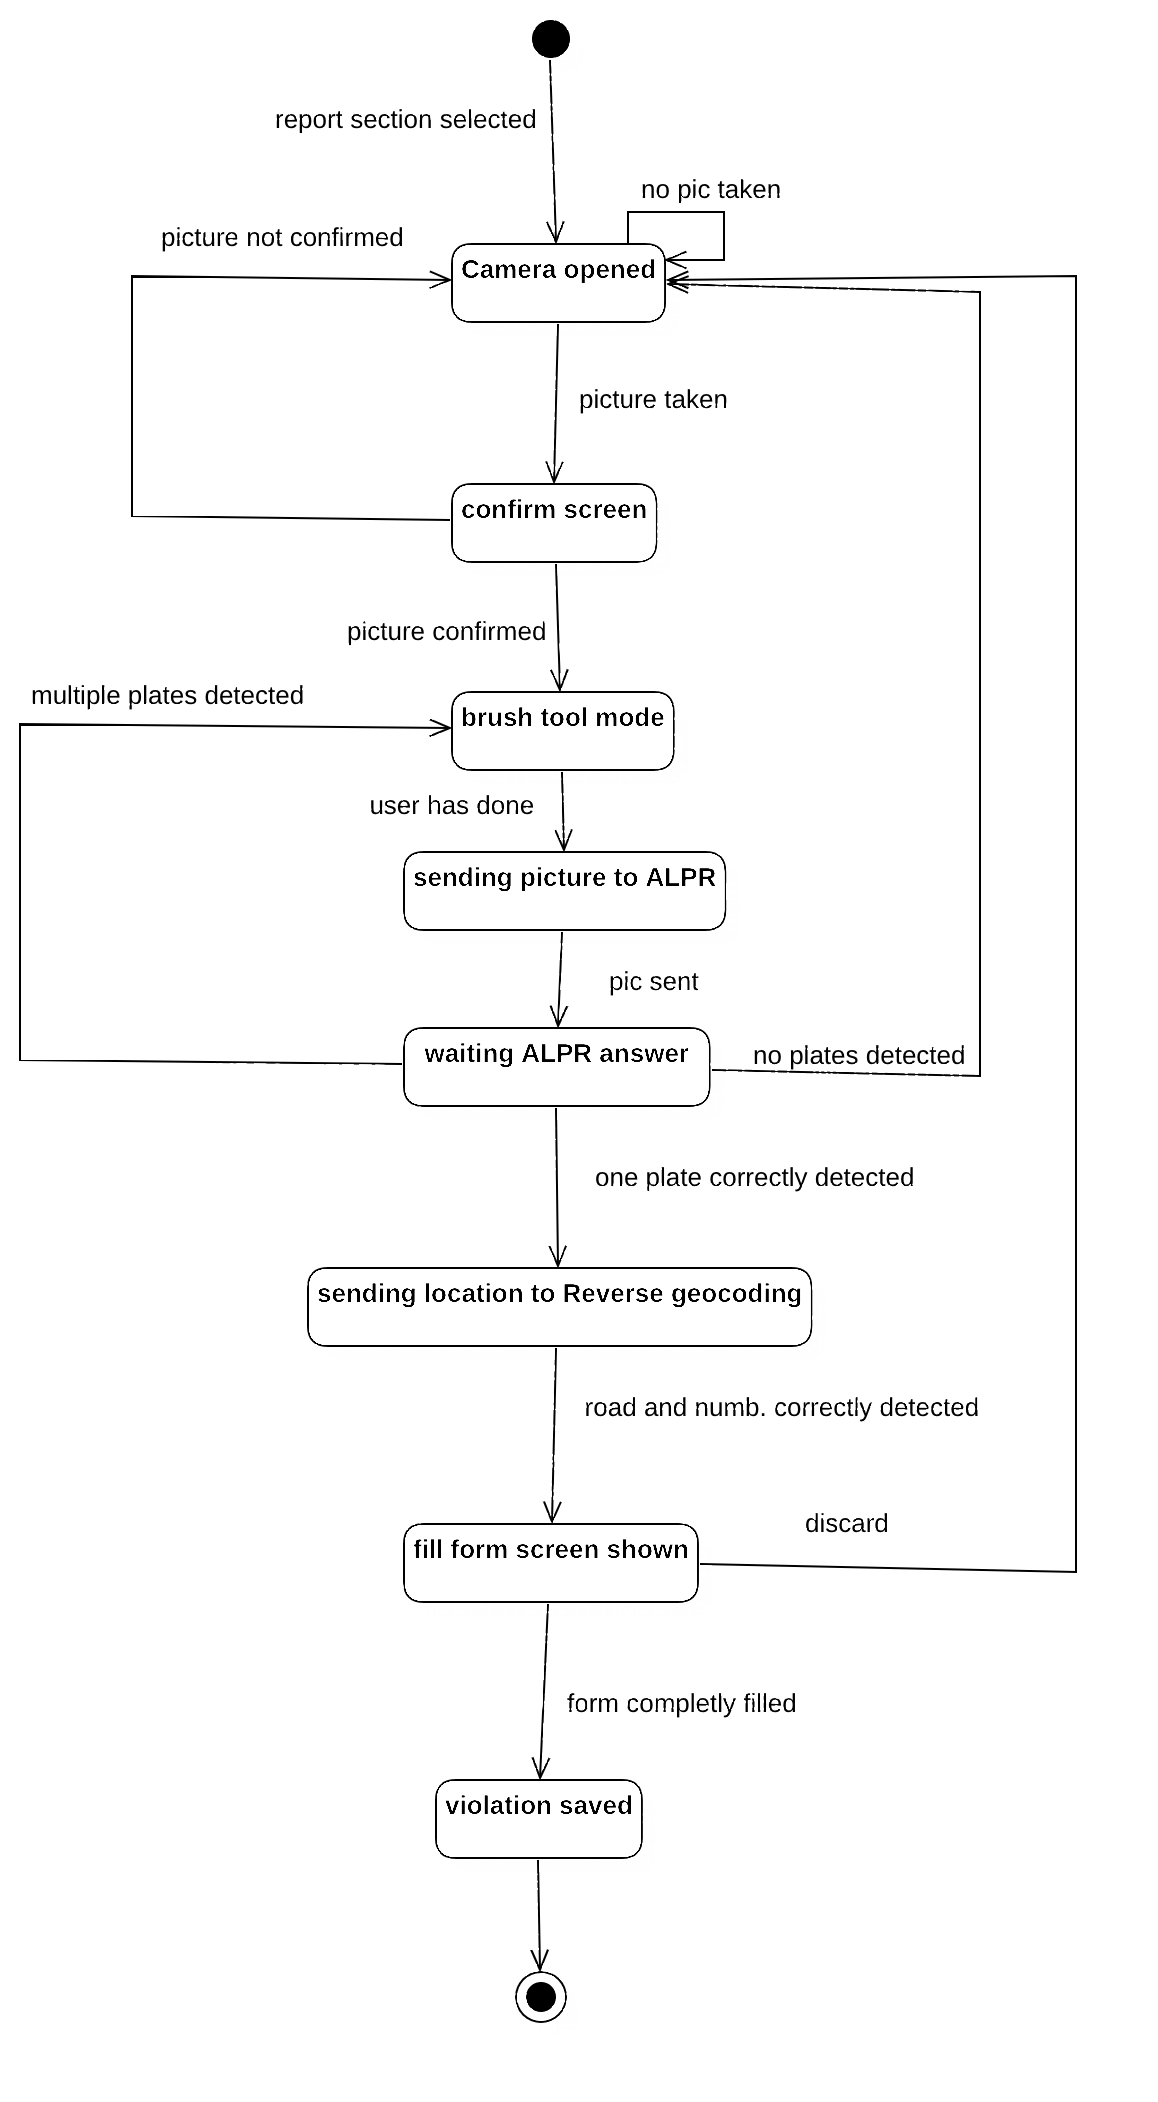
\includegraphics[width=0.7\textwidth]{Images/violationstate.png}
\caption{\label{fig:violationstatediag} Violation reporting state diagram}
\end{figure}

\subsubsection{Explore Data}
\begin{figure}
\centering
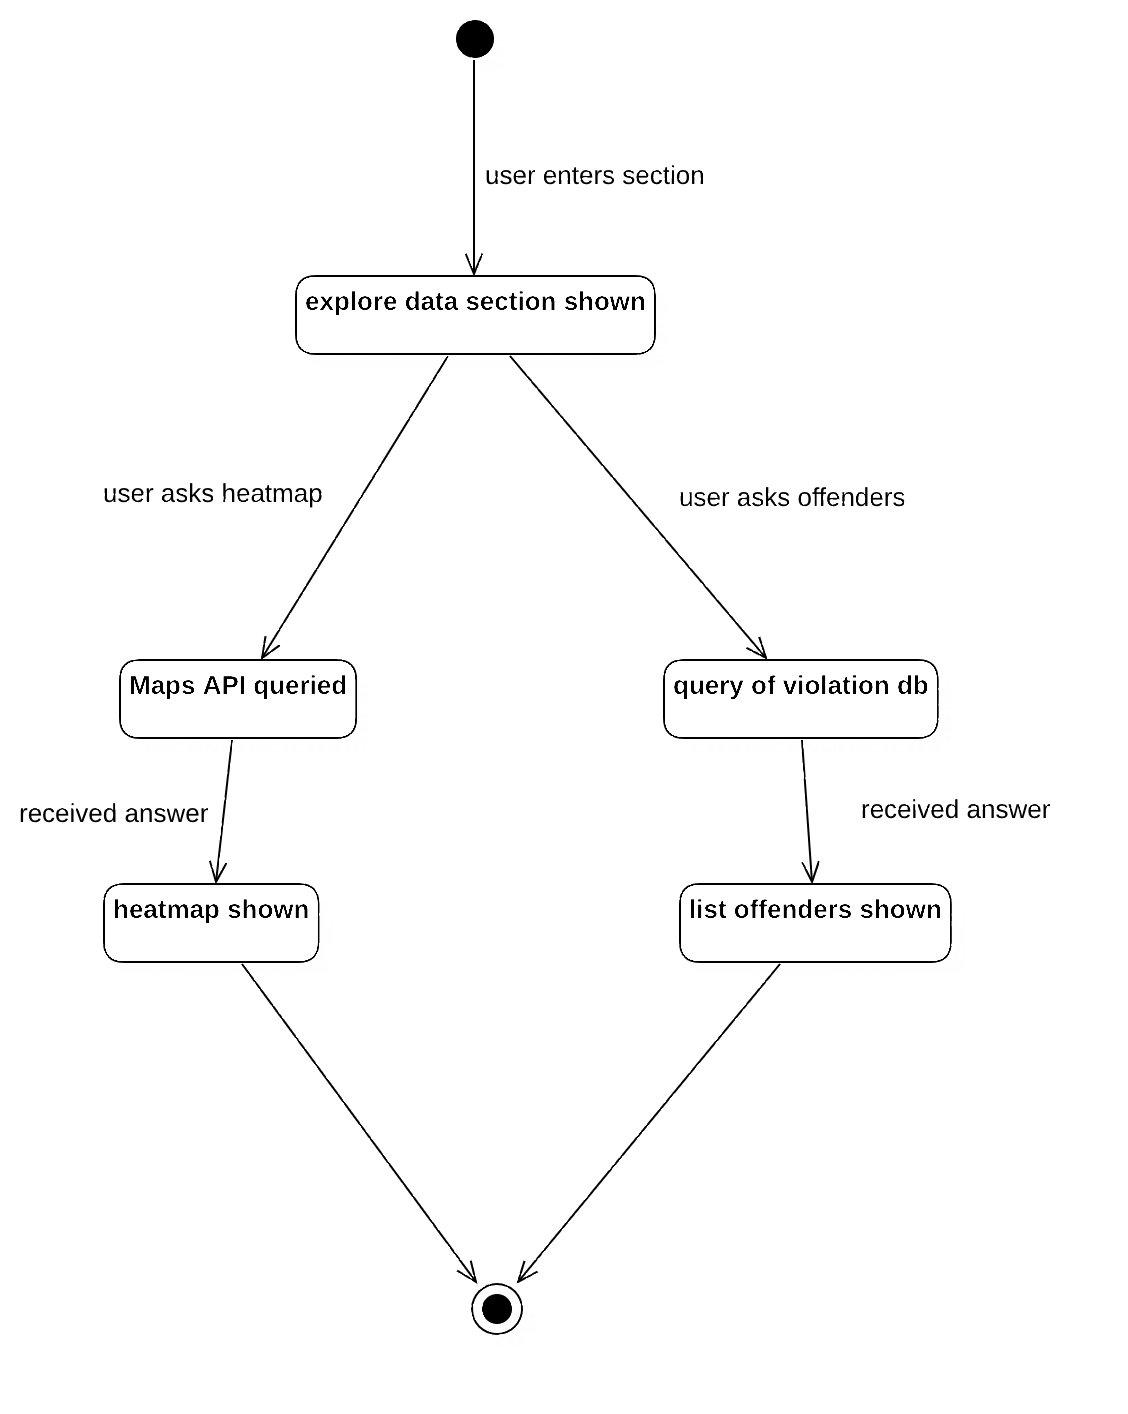
\includegraphics[width=0.7\textwidth]{Images/minestate.png}
\caption{\label{fig:minestatediag} Mining information state diagram}
\end{figure}


The app will offer the possibility to the users to visualize the data collected.
Two kind of visualizations are offered:
\begin{enumerate}
  \item Heatmap of streets where most violations occurred
  \item Vehicles that committed the most violations \label{blacklistplates}
\end{enumerate}
In order to get those data the system will periodically query the database of violations in order to create a table where the count of violation is stored, both for streets and vehicles.
There will be a section in the app called "Explore Data" where will be able to choose which kind of data to visualize.
Only Authority Users will have access to the table of plates which committed the most violations.

\subsubsection{Issue a ticket}

\begin{figure}
\centering
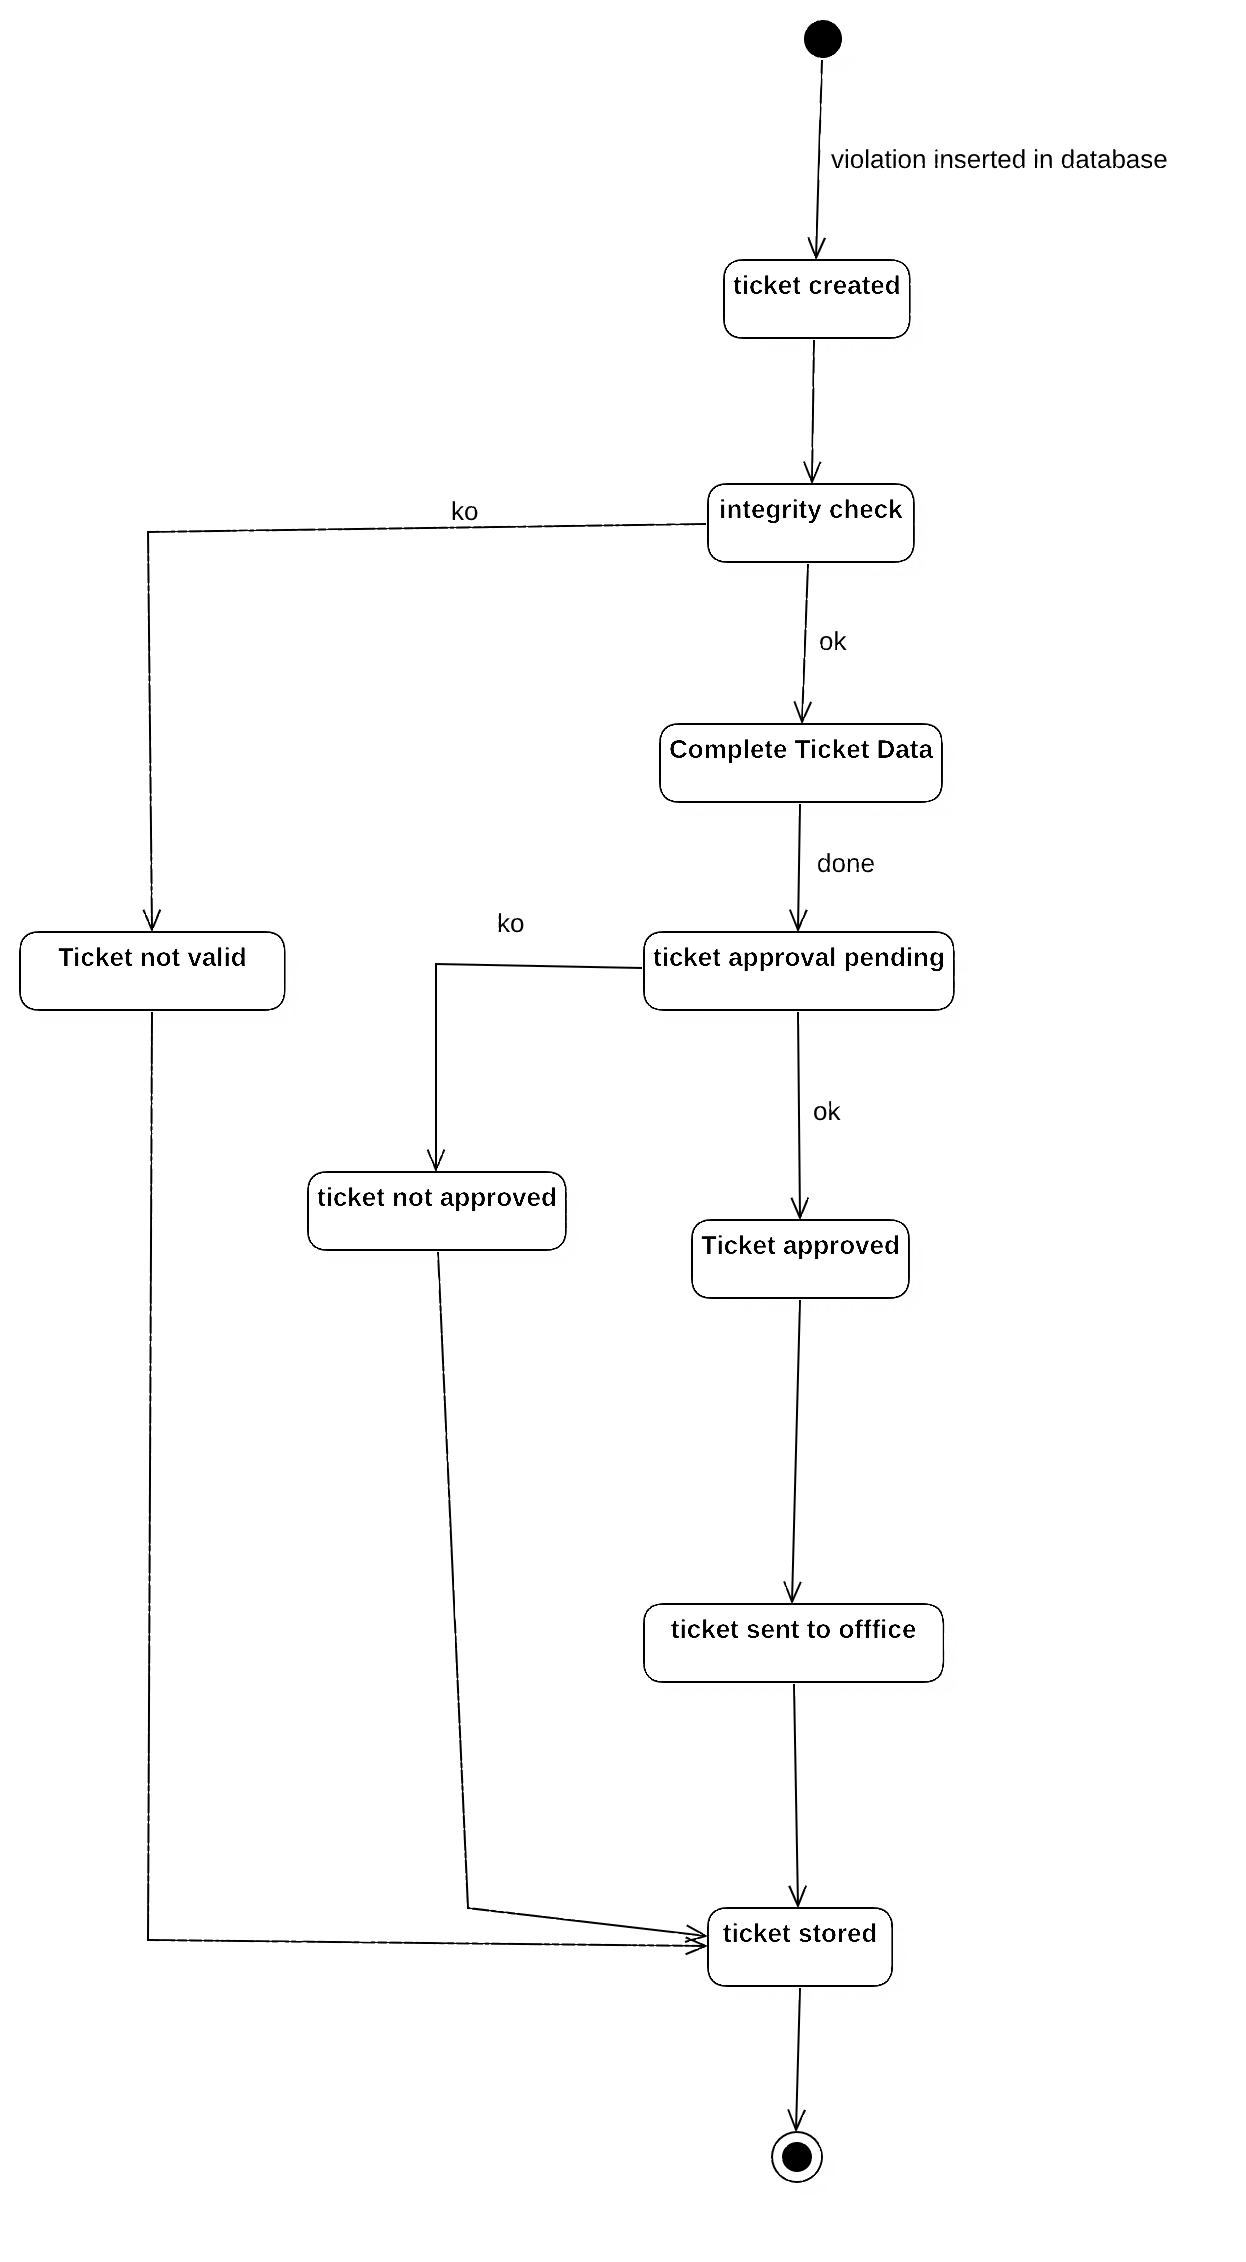
\includegraphics[width=0.7\textwidth]{Images/ticketstate.png}
\caption{\label{fig:ticketstatediag} Tickets creation and approval state diagram}
\end{figure}

This function is used to create tickets to send fines to the owners of vehicles which have been reported by SafeStreets.
Every time a new violation is inserted in the database, the System will use the new data available to generate a proposal of ticket, combining the data from violations with data coming from Municipality databases.

A ticket has the following structure:
\begin{enumerate}
  \item Place where violation occurred
  \item Date when violation occurred
  \item Plate of vehicle
  \item Article and code of violation
  \item Amount to be paid
  \item Date when the payment is due
\end{enumerate}

Place, date, plate are data coming from the instances of Violation class. To create a complete ticket we need to associate the kind of violation to an article and code of the traffic code.

An external service or a piece of software writted ad hoc will be used to check if the picture has been modified.
If the result of this check is positive, the ticket just created will be flagged as \textit{valid} and will go in ticket approval state.
In any other case, which means the picture has been modified, the ticket is stored as \textit{not valid} for debug purposes. Examples of possible uses of those not-valid tickets can be: bulding statistics or investigate if there are users who are trying to cheat or create spam violations.

If a ticket is considered valid, the next state is pending-approval status.
Authority users (e.g. policemen) will check manually the pending-approval tickets reading all data before the approval. We have chosen to add this human control before sending the fine because every ticket should be signed by authorities. If ticket is not approved it will go in approval-denied status and will be stored for debug purposes and for statistics.

If a ticket has been approved it will have to be sent to the offender.
The system will connect to the external vehicle registration database in order to retrieve the name, surname, address of the offender knowing the licence plate of his/her vehicle.
Now we have all the data to print the ticket and send it via regular mail. There will be an office of police-station which will do the job. Maybe in the future tickets will be sent via a Certified E-Mail.

\subsubsection{Ticket statistics}
This function has the purpose to show some statistics about the issued tickets. Here we will take into account only valid and approved tickets.

Two kind of visualizations are offered:
\begin{enumerate}
  \item List of offenders with highest number of tickets emitted
  \item Trends of emitted tickets
\end{enumerate}

Both visualizations will be available only to authorities. In a section of the app it will be possible to see for each citizen who has ever received a ticket the count of those ticket received, in descending order.  Note that this is different compared to the other visulization "vehicles that committed the highest number of violations" explained in section \ref{blacklistplates}.
In this ticket statistic view we are considering only emitted tickets and we are aggregating all tickets of a specific citizen. Actually in case a citizen he has multiple vehicles, here we are counting all the tickets emitted for all of his vehicles.

\subsection{User characteristics}
Here we focus on the needs of our users:
\begin{itemize}
  \item End User : needs an easy and fast way to report violations which must be discrete and effective. this means he can contribute effectively to making the city a better place.
  \item Authorities : they need a service that will help to create tickets, making this process easier. Moreover the ststistics can be used by the municipality to know where there is need to buld more parking areas or improve the local public transport.
  \end{itemize}

\subsection{Assumptions, dependencies and constraints}
\subsubsection{Domain assumptions}

\begin{enumerate}
\dom{1} Device has a working internet connection
\dom{2} Device has a camera accessible via software
\dom{3} The device should acquire position with an accuracy of enough meters in order to univocally determine the road (e.g. 5 meters)
\dom{4} We have access to an ALPR service which is able to read every licence plate in a picture and return each of them as a string
\dom{5} ALPR service has an accuracy of more than 95\%
\dom{6} The device should take pictures with enough resolution to be able to read them with the ALPR service
\dom{7} Every vehicle that can be reported should have a licence plate visible
\dom{8} The number and kind of violations should be finite (defined by the law)
\dom{9} Every authority account is verified and it's not possible to be created using the front end
\dom{10} We have access to the vehicle registration database where are stored licence plates, names and the addresses of the owners of every vehicle registered. Each vehicle has one and only one main owner
\dom{11} We have access to a database where are stored all the codes of violations and the amount of fine for the violation. Every violation has one and only one amount of fine required
\dom{12} The only way to upload pictures of violation is through the application
\dom{13} Each licence plate is unique, there are no vehicles with the same plate

\end{enumerate}

\subsubsection{Dependencies} \label{Dependencies}
Since we're creating a mobile app, the main dependency is to have a smartphone, which has to provide the following features:
\begin{enumerate}
  \item Internet connection, possibly using 2G/3G/4G in order to be available where there is no WiFi, considering the app will be used "on the road"
  \item A camera with good resolution
  \item GPS sensor
\end{enumerate}

Also, there is need to use some external software or APIs :
\begin{itemize}
  \item ALPR service :  the app will be dependent on a third-party service to read the licence plate of the vehicles like the open source OpenALPR \cite{openalprdoc}

  \item Reverse Geocoding: the app will be dependent on some maps API to get the full address, knowing the coordinates of location coming from the GPS of the device. An example of this service is Google Maps API \cite{GMapGeocode}

  \item Map and Heatmap : The app will be dependent to some Maps API used to show the map with an overlay. An example of this service is Google Maps API \cite{GMapsHeat}
\end{itemize}
